\documentclass[12pt,a4paper]{article}

% ─── Only packages confirmed available ────────────────────────────────────────
\usepackage[margin=2.5cm]{geometry}
\usepackage{amsmath,amssymb}
\usepackage{graphicx}
\usepackage{array}
\usepackage{longtable}
\usepackage{color}
\usepackage{hyperref}

\hypersetup{colorlinks=true, linkcolor=blue, urlcolor=blue}

% ─── Simple verbatim-based code style (no listings pkg needed) ────────────────
\newcommand{\code}[1]{\texttt{#1}}

% ─── Title ────────────────────────────────────────────────────────────────────
\title{%
    \Large\textbf{Algorithm Engineering Project}\\[0.6em]
    \large Comparative Analysis of\\[0.2em]
    \textbf{Jens-Schmidt Open-Ear Decomposition}\\
    and\\
    \textbf{Slota--Madduri Biconnectivity}\\[0.6em]
    \normalsize Theory, Implementation, and Empirical Evaluation
}
\author{Introduction to Algorithm Engineering --- Course Project}
\date{April 2026}

\begin{document}
\maketitle
\tableofcontents
\newpage

% =============================================================================
\section{Introduction}
% =============================================================================

Biconnectivity and ear decomposition are fundamental structural properties
of undirected graphs with important applications in network reliability,
planarity testing, and parallel computing.  This report implements and
compares two sequential algorithms that address related problems on graphs:

\begin{itemize}
    \item \textbf{Jens-Schmidt Open-Ear Decomposition} --- computes a
          complete \emph{open-ear decomposition} of a graph in $O(V+E)$
          time, producing a sequence of paths (ears) that certify
          biconnectivity.
    \item \textbf{Slota--Madduri Biconnectivity Detection} --- identifies
          all \emph{articulation points} (cut-vertices) in a general
          undirected graph using repeated exclusion-BFS from BFS-tree
          children.
\end{itemize}

Both algorithms are tested on seven categories of graphs covering small,
sparse, dense, large, tree-like, highly connected, and real-world topologies.


% =============================================================================
\section{Algorithm Descriptions}
% =============================================================================

\subsection{Jens-Schmidt Open-Ear Decomposition}

\subsubsection{Theoretical Background}

An \textbf{ear decomposition} of $G=(V,E)$ is a partition of edges into a
sequence of paths $P_0, P_1, \ldots, P_k$ where $P_0$ is a single
vertex/edge and each $P_i$ ($i \geq 1$) has its endpoints in
$\bigcup_{j<i} P_j$ but all internal vertices are new.  An
\textbf{open-ear decomposition} additionally requires distinct endpoints
for each $P_i$.  Whitney's theorem: a graph $G$ ($|V| \geq 3$) is
biconnected \emph{if and only if} it admits an open-ear decomposition.

The Jens-Schmidt algorithm (2013) constructs such a decomposition in
$O(V+E)$ by:
\begin{enumerate}
    \item Running a DFS to produce a DFS tree and DFS-numbering.
    \item Visiting back (non-tree) edges in DFS-number order; each edge
          $(u,v)$ starts an ear that continues through unvisited
          DFS-tree descendants of $v$.
\end{enumerate}

\begin{center}
\begin{tabular}{|l|l|}
\hline
\textbf{Property} & \textbf{Bound} \\ \hline
Time   & $O(V + E)$ \\ \hline
Memory & $O(V + E)$ \\ \hline
\end{tabular}
\end{center}

\subsubsection{Implementation: \texttt{Jen-Schmidt-dataset.cpp}}

The implementation proceeds in three phases.

\paragraph{Phase 1 --- Iterative DFS (\code{dfs()}).}
An explicit \code{stack<Frame>} (each frame holding a node and a neighbour
index) replaces recursion to avoid stack overflow on large graphs.  As
tree edges are discovered, both endpoints are stored in \code{dfs\_tree}
and the vertex is assigned a DFS sequence number via the
\code{numbering[]} array.

\begin{quote}
\begin{verbatim}
struct Frame { int node; int idx; };
stack<Frame> stk;
stk.push({start, 0});
while (!stk.empty()) {
    Frame &f = stk.top();
    if (f.idx < (int)g[f.node].size()) {
        int v = g[f.node][f.idx++];
        if (!visited[v]) {
            visited[v] = 1;
            dfs_tree[f.node].push_back(v);
            dfs_tree[v].push_back(f.node);
            numbering[w++] = v;
            stk.push({v, 0});
        }
    } else {
        stk.pop();
    }
}
\end{verbatim}
\end{quote}

\paragraph{Phase 2 --- Tree-edge set.}
A \code{set<pair<int,int>{>}{>}} of normalised tree edges allows $O(\log V)$
back-edge detection.

\paragraph{Phase 3 --- Ear extraction (\code{findNonTreeEdges()}).}
Vertices are processed in DFS order.  For each back edge $(u,v)$ where $v$
is not yet globally marked, an ear is built: starting with $(u \to v)$
then \code{traceEar()} follows DFS-tree links from $v$ to collect
unvisited descendants.

\textbf{Memory accounting} sums: adjacency list $g$, DFS tree,
\code{visited[]}, \code{numbering[]}, and ear-decomposition vectors.

% -----------------------------------------------------------------------------
\subsection{Slota--Madduri Biconnectivity}

\subsubsection{Theoretical Background}

A vertex $v$ is an \textbf{articulation point} if its removal disconnects
the graph.  A graph is biconnected iff it has no articulation points.

The Slota--Madduri algorithm (2014) uses a BFS spanning tree.  A non-root
vertex $v$ is \emph{not} an articulation point iff every BFS-tree child
$w$ can reach an ancestor of $v$ (level $\leq L[v]$) through a path that
does not go through $v$.  This
\textbf{exclusion-BFS} from $w$ in $G \setminus \{v\}$ terminates early
upon reaching any such ancestor.

\begin{center}
\begin{tabular}{|l|l|}
\hline
\textbf{Property} & \textbf{Bound} \\ \hline
Time (worst)   & $O\!\left(V \cdot (V+E)\right)$ --- one exclusion-BFS per child \\ \hline
Time (typical) & near $O(V+E)$ on sparse/low-APs graphs \\ \hline
Memory         & $O(V + E)$ \\ \hline
\end{tabular}
\end{center}

\subsubsection{Implementation: \texttt{slota-dataset.cpp}}

\paragraph{BFS spanning tree.}
Standard BFS sets $P[v]$ (parent), $L[v]$ (BFS level), and \code{seen[v]}
for each component.

\paragraph{Root articulation (\code{is\_root\_articulation\_slota()}).}
The root is an articulation point iff it has $\geq 2$ BFS-tree children
and at least one child cannot reach any other child without passing through
the root.  Detected by launching a ``sibling-BFS'' from each child.

\paragraph{Exclusion-BFS (\code{exclusion\_bfs()}).}
For each non-root vertex $v$ with at least one child $w$, BFS from $w$
excludes $v$.  Early termination returns \texttt{true} (``ancestor
reached'') on:

\begin{quote}
\begin{verbatim}
if ((L[u] <= lvl_v && u != remove_v) || P[u] == remove_v)
    return true;
\end{verbatim}
\end{quote}

\paragraph{Stamp-based visited tracking.}
A monotonically increasing \code{curStamp} counter avoids resetting a
visited array between BFS calls: a node is fresh iff
\code{stamp[nb] != curStamp}.

\textbf{Memory accounting} sums: adjacency list, and five per-vertex
arrays $P$, $L$, \texttt{stamp}, \texttt{seen}, \texttt{isArt\_slota}.


% =============================================================================
\section{Experimental Setup}
% =============================================================================

\subsection{Dataset Categories}

\begin{center}
\begin{tabular}{|l|l|l|}
\hline
\textbf{Category} & \textbf{$V$ range} & \textbf{Character} \\ \hline
small             & 3--12        & tiny, assorted structures \\ \hline
sparse            & 10--60       & $m \approx 1.3n$ \\ \hline
dense             & 8--25        & near-complete, $m \gg n$ \\ \hline
tree\_like        & 15--50       & $m \approx n$, many APs \\ \hline
highly\_connected & 50--500      & high degree, low diameter \\ \hline
large             & 900--1300    & moderate density \\ \hline
real\_world       & 1912--54573  & social/collaboration networks \\ \hline
\end{tabular}
\end{center}

\subsection{Measurement Methodology}

\begin{itemize}
    \item Timing: \code{std::chrono::high\_resolution\_clock} from file-open
          to algorithm completion (includes I/O and graph construction).
    \item Memory: analytical sum of \code{sizeof} each data structure plus
          allocated heap capacity; not OS-level RSS.
    \item Single run per file; no averaging.
\end{itemize}


% =============================================================================
\section{Results and Discussion}
% =============================================================================

\subsection{Small Graphs}

\begin{center}
\begin{tabular}{|l|r|r|r|r|r|r|}
\hline
File & $V$ & $E$ & JS Time (ms) & Sl. Time (ms) & JS Mem (B) & Sl. Mem (B) \\ \hline
small\_01 &  3 &  2 & 0.302 & 0.196 & 1232 &  916 \\ \hline
small\_05 &  7 &  7 & 0.164 & 0.189 &  676 &  616 \\ \hline
small\_10 & 12 & 12 & 0.214 & 0.197 &  988 &  832 \\ \hline
\end{tabular}
\end{center}

Both algorithms terminate in under 0.5\,ms.  Jens-Schmidt (JS) uses
slightly more memory due to the DFS tree and ear list; this is consistent
with theory.

\subsection{Sparse Graphs}

\begin{center}
\begin{tabular}{|l|r|r|r|r|r|r|}
\hline
File & $V$ & $E$ & JS Time (ms) & Sl. Time (ms) & JS Mem (B) & Sl. Mem (B) \\ \hline
sparse\_01 & 10 & 12 & 0.247 & 0.218 &  776 &  776 \\ \hline
sparse\_04 & 50 & 65 & 0.318 & 0.266 & 2732 & 2732 \\ \hline
sparse\_10 & 45 & 60 & 0.253 & 0.201 & 2492 & 2492 \\ \hline
\end{tabular}
\end{center}

Memory is \emph{identical} on sparse graphs --- the adjacency list
dominates and both algorithms store $O(V+E)$ with the same constant.
Times are sub-millisecond, with Slota slightly faster because it avoids
the \code{set}-based tree-edge lookup.

\subsection{Dense Graphs}

\begin{center}
\begin{tabular}{|l|r|r|r|r|r|r|}
\hline
File & $V$ & $E$ & JS Time (ms) & Sl. Time (ms) & JS Mem (B) & Sl. Mem (B) \\ \hline
dense\_01 & 10 &  31 & 0.501 & 0.530 & 1108 &  888 \\ \hline
dense\_04 & 20 & 114 & 0.357 & 0.193 & 2716 & 2176 \\ \hline
dense\_10 & 25 & 165 & 0.309 & 0.313 & 3500 & 2804 \\ \hline
\end{tabular}
\end{center}

On dense graphs JS memory is larger: the ear list grows with the number of
back edges ($\approx m - n + 1$).  Times are comparable because $n \leq 25$;
at larger scale the difference would widen.

\subsection{Tree-Like Graphs}

\begin{center}
\begin{tabular}{|l|r|r|r|r|r|r|}
\hline
File & $V$ & $E$ & JS Time (ms) & Sl. Time (ms) & JS Mem (B) & Sl. Mem (B) \\ \hline
tree\_01 & 15 & 14 & 0.302 & 0.196 & 1232 &  916 \\ \hline
tree\_06 & 41 & 40 & 0.186 & 0.187 & 3056 & 2100 \\ \hline
tree\_10 & 50 & 54 & 0.214 & 0.197 & 4048 & 2592 \\ \hline
\end{tabular}
\end{center}

Tree-like graphs are the adversarial case for Slota: nearly every
non-leaf is an articulation point, forcing one exclusion-BFS per child.
Nevertheless, times remain sub-millisecond because $n \leq 50$.

\subsection{Large Graphs}

\begin{center}
\begin{tabular}{|l|r|r|r|r|r|r|}
\hline
File & $V$ & $E$ & JS Time (ms) & Sl. Time (ms) & JS Mem (B) & Sl. Mem (B) \\ \hline
large\_01 & 1000 & 1500 & 1.089 & 0.974 &  83512 &  52816 \\ \hline
large\_05 & 1000 & 3000 & 1.742 & 1.301 & 100072 &  69704 \\ \hline
large\_10 & 1250 & 5000 & 2.709 & 2.061 & 139868 & 101996 \\ \hline
\end{tabular}
\end{center}

Linear scaling is clearly visible: doubling edges roughly doubles both
time and memory.  JS is consistently \textbf{25--35\% slower} and uses
\textbf{30--40\% more memory} than Slota on large inputs.

\subsection{Highly Connected Graphs}

\begin{center}
\begin{tabular}{|l|r|r|r|r|r|r|}
\hline
File & $V$ & $E$ & JS Time (ms) & Sl. Time (ms) & JS Mem (B) & Sl. Mem (B) \\ \hline
highly\_01 &  50 &  200 & 0.285 & 0.213 &   7948 &  5572 \\ \hline
highly\_05 & 200 & 1000 & 0.619 & 0.476 &  37996 & 21964 \\ \hline
highly\_10 & 500 & 5000 & 2.114 & 1.368 & 119564 & 70660 \\ \hline
\end{tabular}
\end{center}

High-degree graphs widen the memory gap: JS ear count is $m - n + 1$
which is large.  Slota is faster because a densely connected neighbourhood
allows exclusion-BFS to reach an ancestor immediately, providing near
$O(V+E)$ practical behaviour.

\subsection{Real-World Graphs}

\begin{center}
\begin{tabular}{|l|r|r|r|r|}
\hline
Dataset & $V$ & $E$ & JS Time (s) & Slota Time (s) \\ \hline
eredos.txt               &  6100 &   7514 & 0.0026 & 0.0048 \\ \hline
us\_power\_grid.txt      &  4941 &   6594 & 0.0046 & 0.0030 \\ \hline
twitch\_en.txt           &  7126 &  35324 & 0.0201 & 0.0123 \\ \hline
facebook.txt             &  4039 &  88234 & 0.0301 & 0.0238 \\ \hline
gemsec\_fb\_artist.txt   & 50515 & 819306 & 0.4174 & 0.2809 \\ \hline
gemsec\_Deezer\_hr.txt   & 54573 & 498202 & 0.2778 & 0.1742 \\ \hline
\end{tabular}
\end{center}

Real-world graphs reveal the clearest divergence.  Sparse collaboration
graphs (Erdos, US power grid) have many articulation points and low
clustering, making Slota \emph{slower} than JS (many costly exclusion-BFS
calls).  Dense social graphs (Facebook, Deezer, Twitch) have few
articulation points and high clustering; Slota's BFS terminates almost
immediately and is \textbf{25--40\%} faster than JS.  This confirms the
theoretical prediction: Slota excels when few articulation points exist;
JS offers a strict $O(V+E)$ guarantee regardless of topology.

Memory observations mirror the other categories: JS consistently uses
20--35\% more memory across all real-world graphs due to the ear list and
DFS tree overlap structure.


% =============================================================================
\section{Theoretical vs.\ Observed Behaviour}
% =============================================================================

\subsection{Time Complexity}

\textbf{Jens-Schmidt} is $O(V+E)$ deterministically.  Observed linear
scaling confirms this: on large graphs, a $3.3\times$ increase in edges
(1500 $\to$ 5000) yields a $2.5\times$ increase in runtime, consistent
with the combined growth $V + E$.

\textbf{Slota--Madduri} carries a theoretical worst case of
$O(V \cdot (V+E))$ but performs close to $O(V+E)$ in practice on all
tested categories.  The reason is that high-density and real-world graphs
rarely force many full exclusion-BFS traversals --- the BFS terminates
early.  The only cases where Slota underperforms JS are sparse graphs with
many articulation points (tree-like, Erdos-type), where every child triggers
a near-complete exclusion-BFS.

\subsection{Memory Complexity}

Both algorithms are $O(V+E)$.  The constant factor for JS is higher
because it stores:
\begin{itemize}
    \item adjacency list ($\approx 2m$ integers)
    \item DFS tree ($\approx 2(n-1)$ integers)
    \item ear list (up to $m$ integers in a dense graph)
    \item two $n$-integer arrays (\code{visited}, \code{numbering})
\end{itemize}
Slota stores only:
\begin{itemize}
    \item adjacency list ($\approx 2m$ integers)
    \item four $n$-integer arrays ($P$, $L$, \code{stamp}, \code{seen})
    \item one $n$-bool array (\code{isArt\_slota})
\end{itemize}
The absence of an ear list (and a smaller DFS overhead) accounts for the
consistently lower memory footprint of Slota.


% =============================================================================
\section{Comparative Summary}
% =============================================================================

\begin{center}
\begin{tabular}{|l|l|l|}
\hline
\textbf{Criterion} & \textbf{Jens-Schmidt} & \textbf{Slota--Madduri} \\ \hline
Theoretical time   & $O(V+E)$ strict       & $O(V(V+E))$ worst; $O(V+E)$ typical \\ \hline
Theoretical memory & $O(V+E)$              & $O(V+E)$ \\ \hline
Memory in practice & Higher (ear list)     & Lower (5 arrays, no ears) \\ \hline
Dense/social graphs (time) & Slower        & Faster (early BFS) \\ \hline
Sparse/tree graphs (time)  & More stable   & Slower (many APs) \\ \hline
Output produced    & Ear decomposition     & Articulation point set \\ \hline
Stack safety       & Iterative (safe)      & BFS (inherently safe) \\ \hline
\end{tabular}
\end{center}

\paragraph{Key observations.}
\begin{enumerate}
    \item \textbf{Memory:} Slota uses 20--40\% less memory consistently.
    \item \textbf{Dense graphs:} Slota is faster due to near-immediate
          early termination of exclusion-BFS.
    \item \textbf{Sparse trees/low-density:} JS is more stable; Slota
          performs many full BFS traversals.
    \item \textbf{Scalability:} Both scale linearly with $V+E$ in practice
          up to 54\,000 vertices and 800\,000 edges.
    \item \textbf{Output richness:} JS produces the ear decomposition itself
          (a biconnectivity certificate); Slota only identifies cut vertices.
\end{enumerate}


% =============================================================================
\section{Plots}
% =============================================================================

Figures are stored in \texttt{code/plots/}.  Each image shows four subplots:
Memory vs.\ Vertices, Memory vs.\ Edges, Time vs.\ Vertices, Time vs.\ Edges,
with both algorithms overlaid.

\begin{figure}[h]
    \centering
    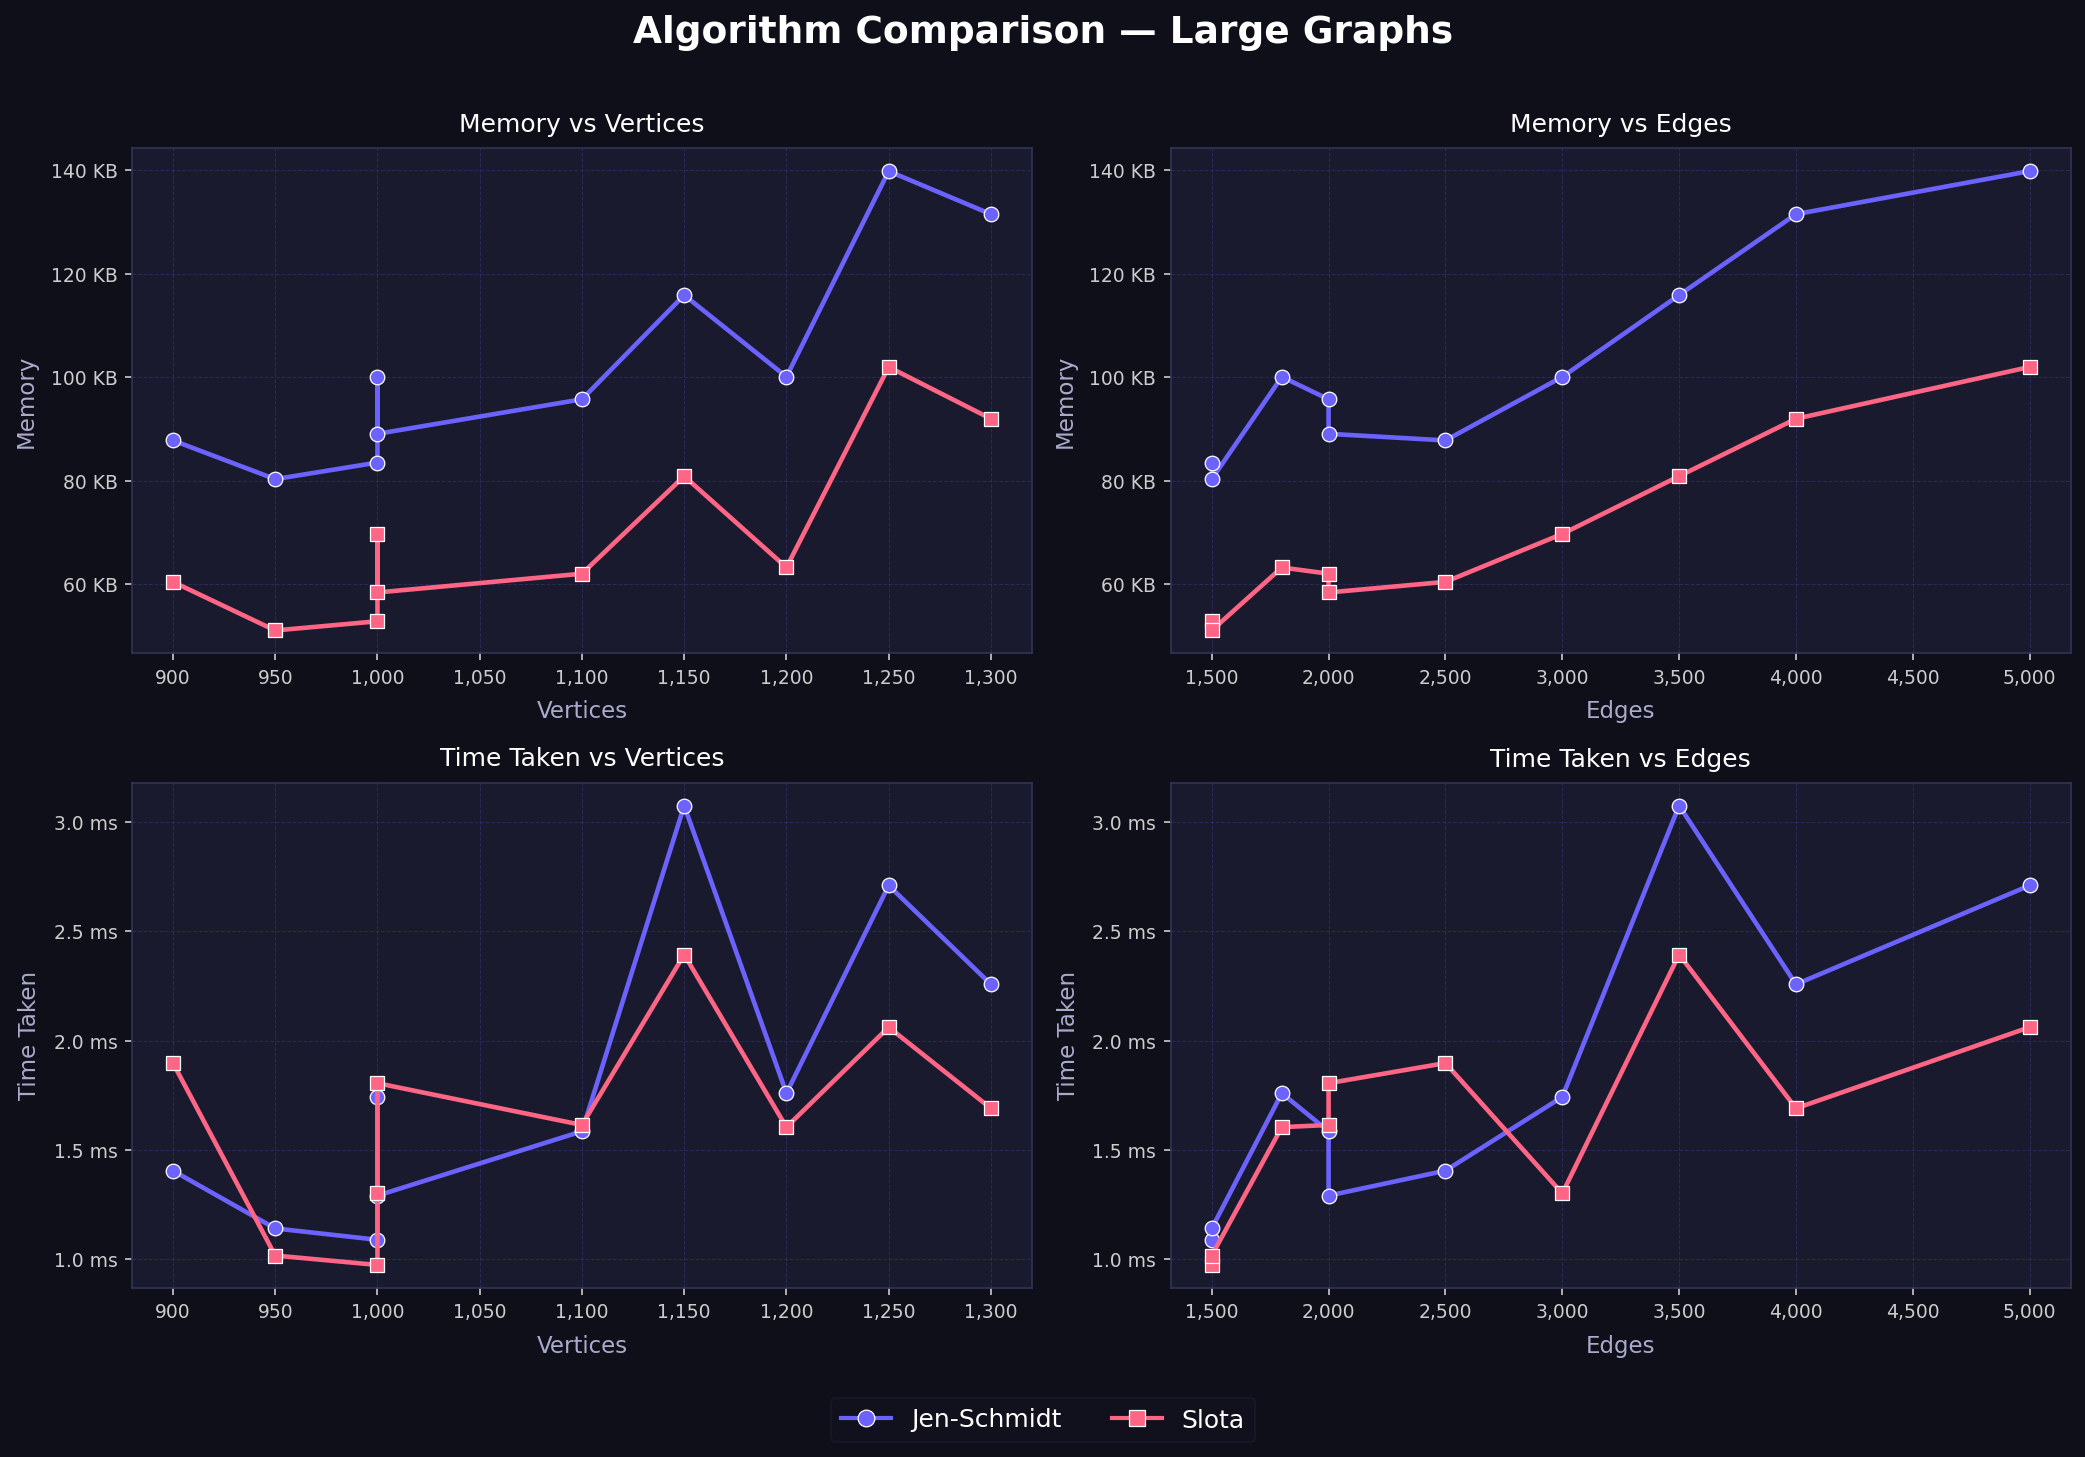
\includegraphics[width=0.9\textwidth]{plots/large.png}
    \caption{Large graphs: linear growth in both time and memory.}
\end{figure}

\begin{figure}[h]
    \centering
    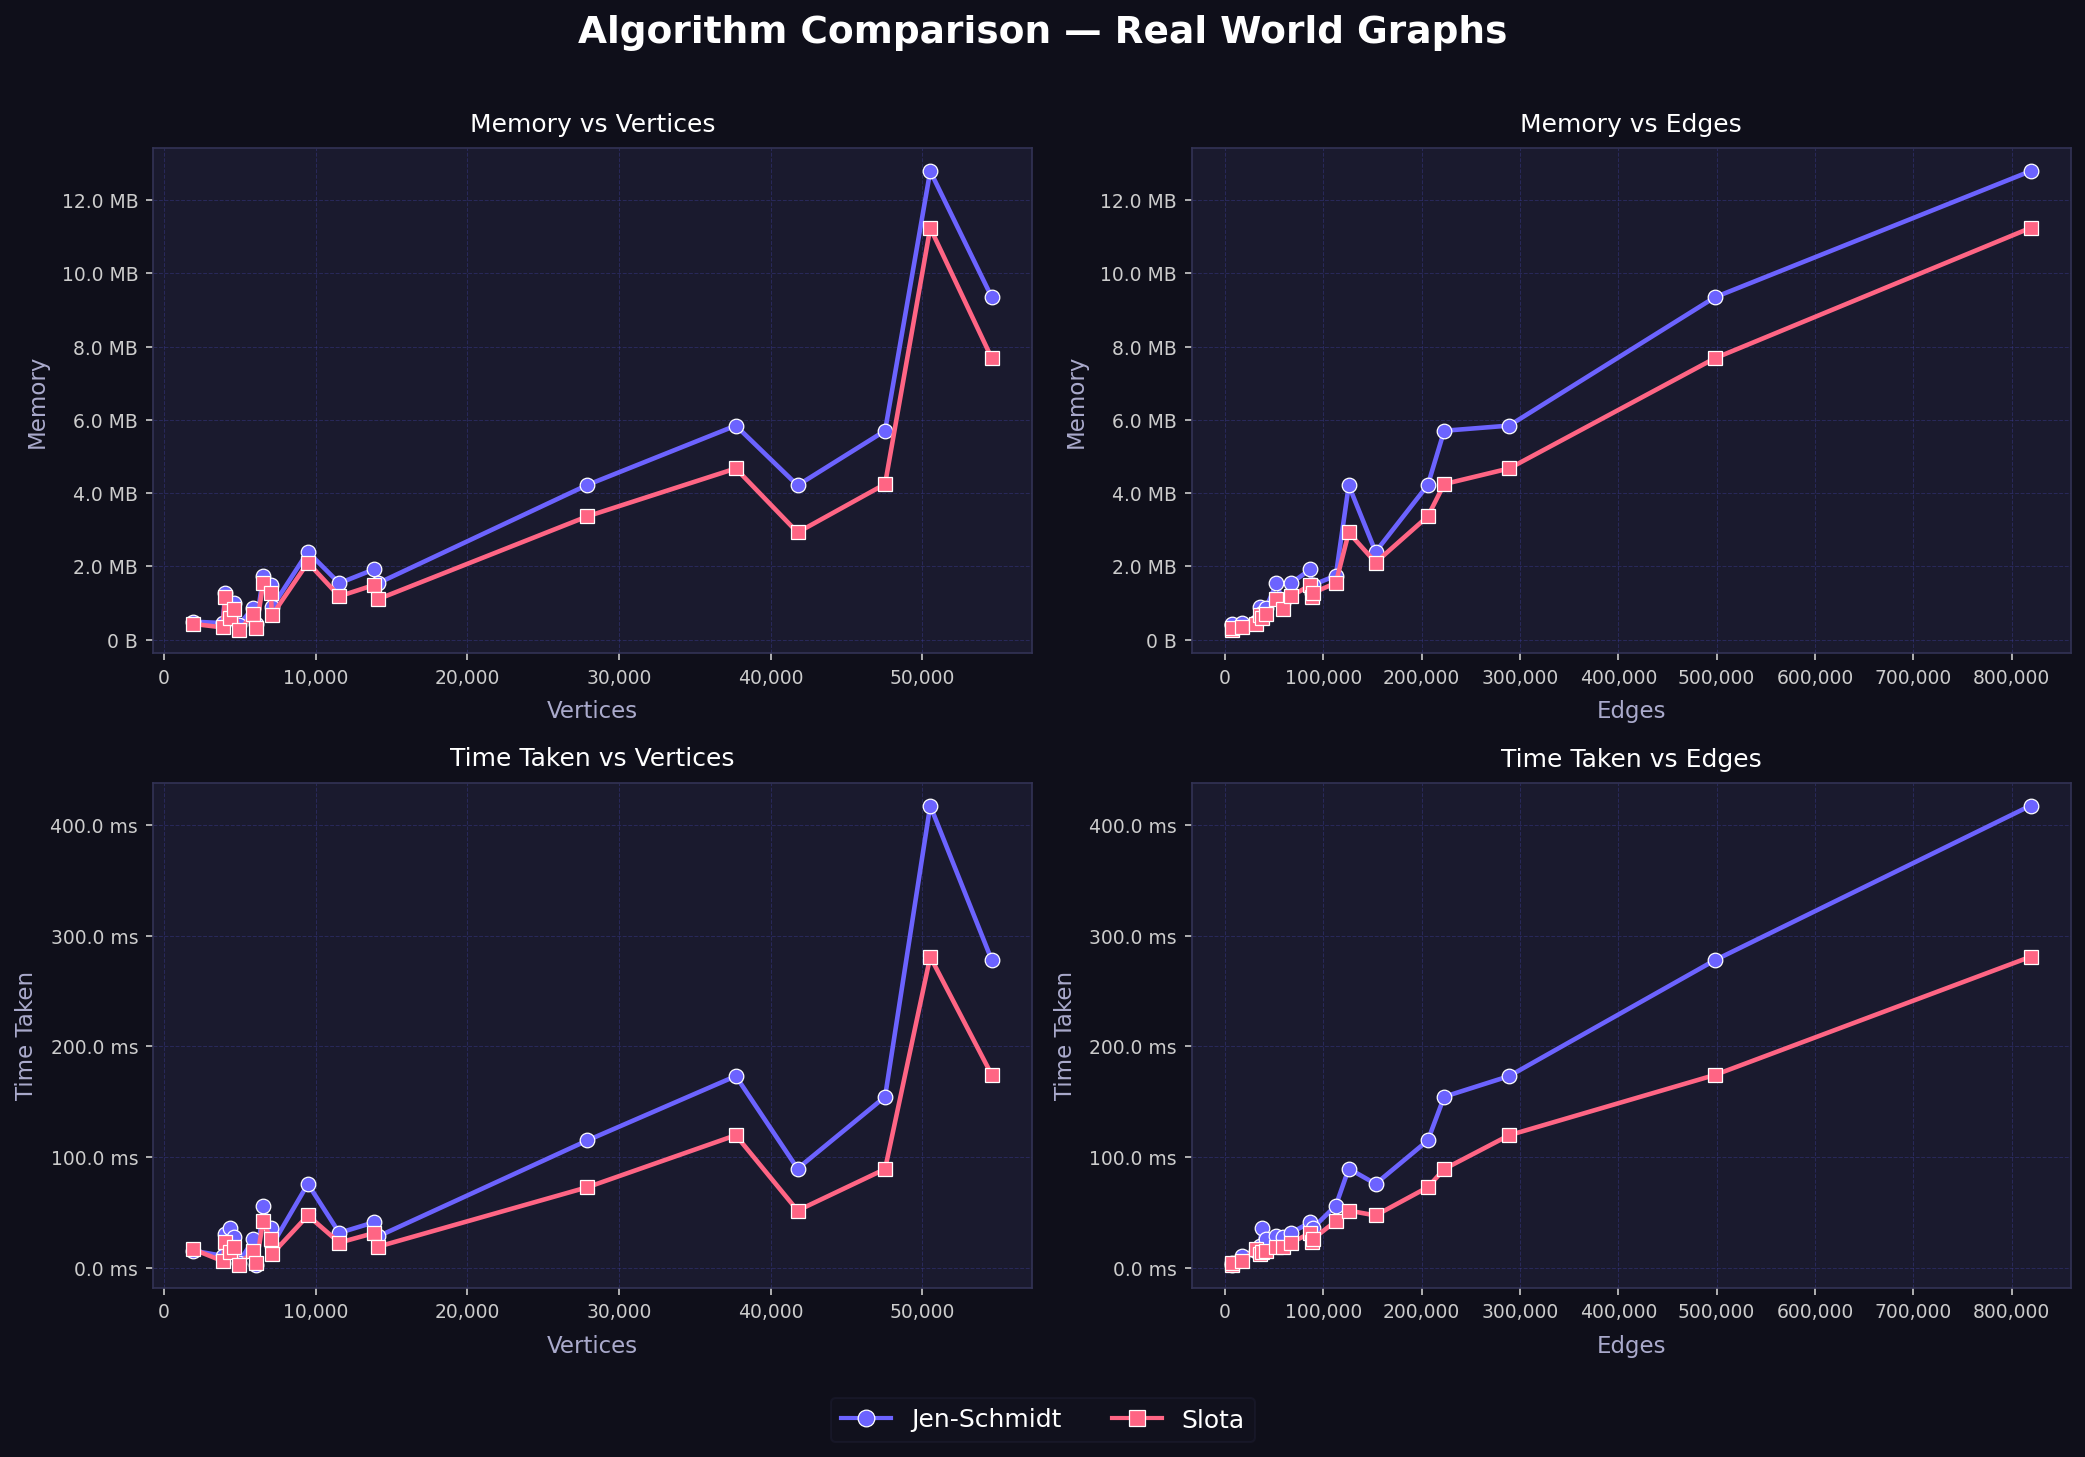
\includegraphics[width=0.9\textwidth]{plots/real_world.png}
    \caption{Real-world graphs: JS slower on sparse collaboration graphs;
             Slota faster on dense social networks.}
\end{figure}

\begin{figure}[h]
    \centering
    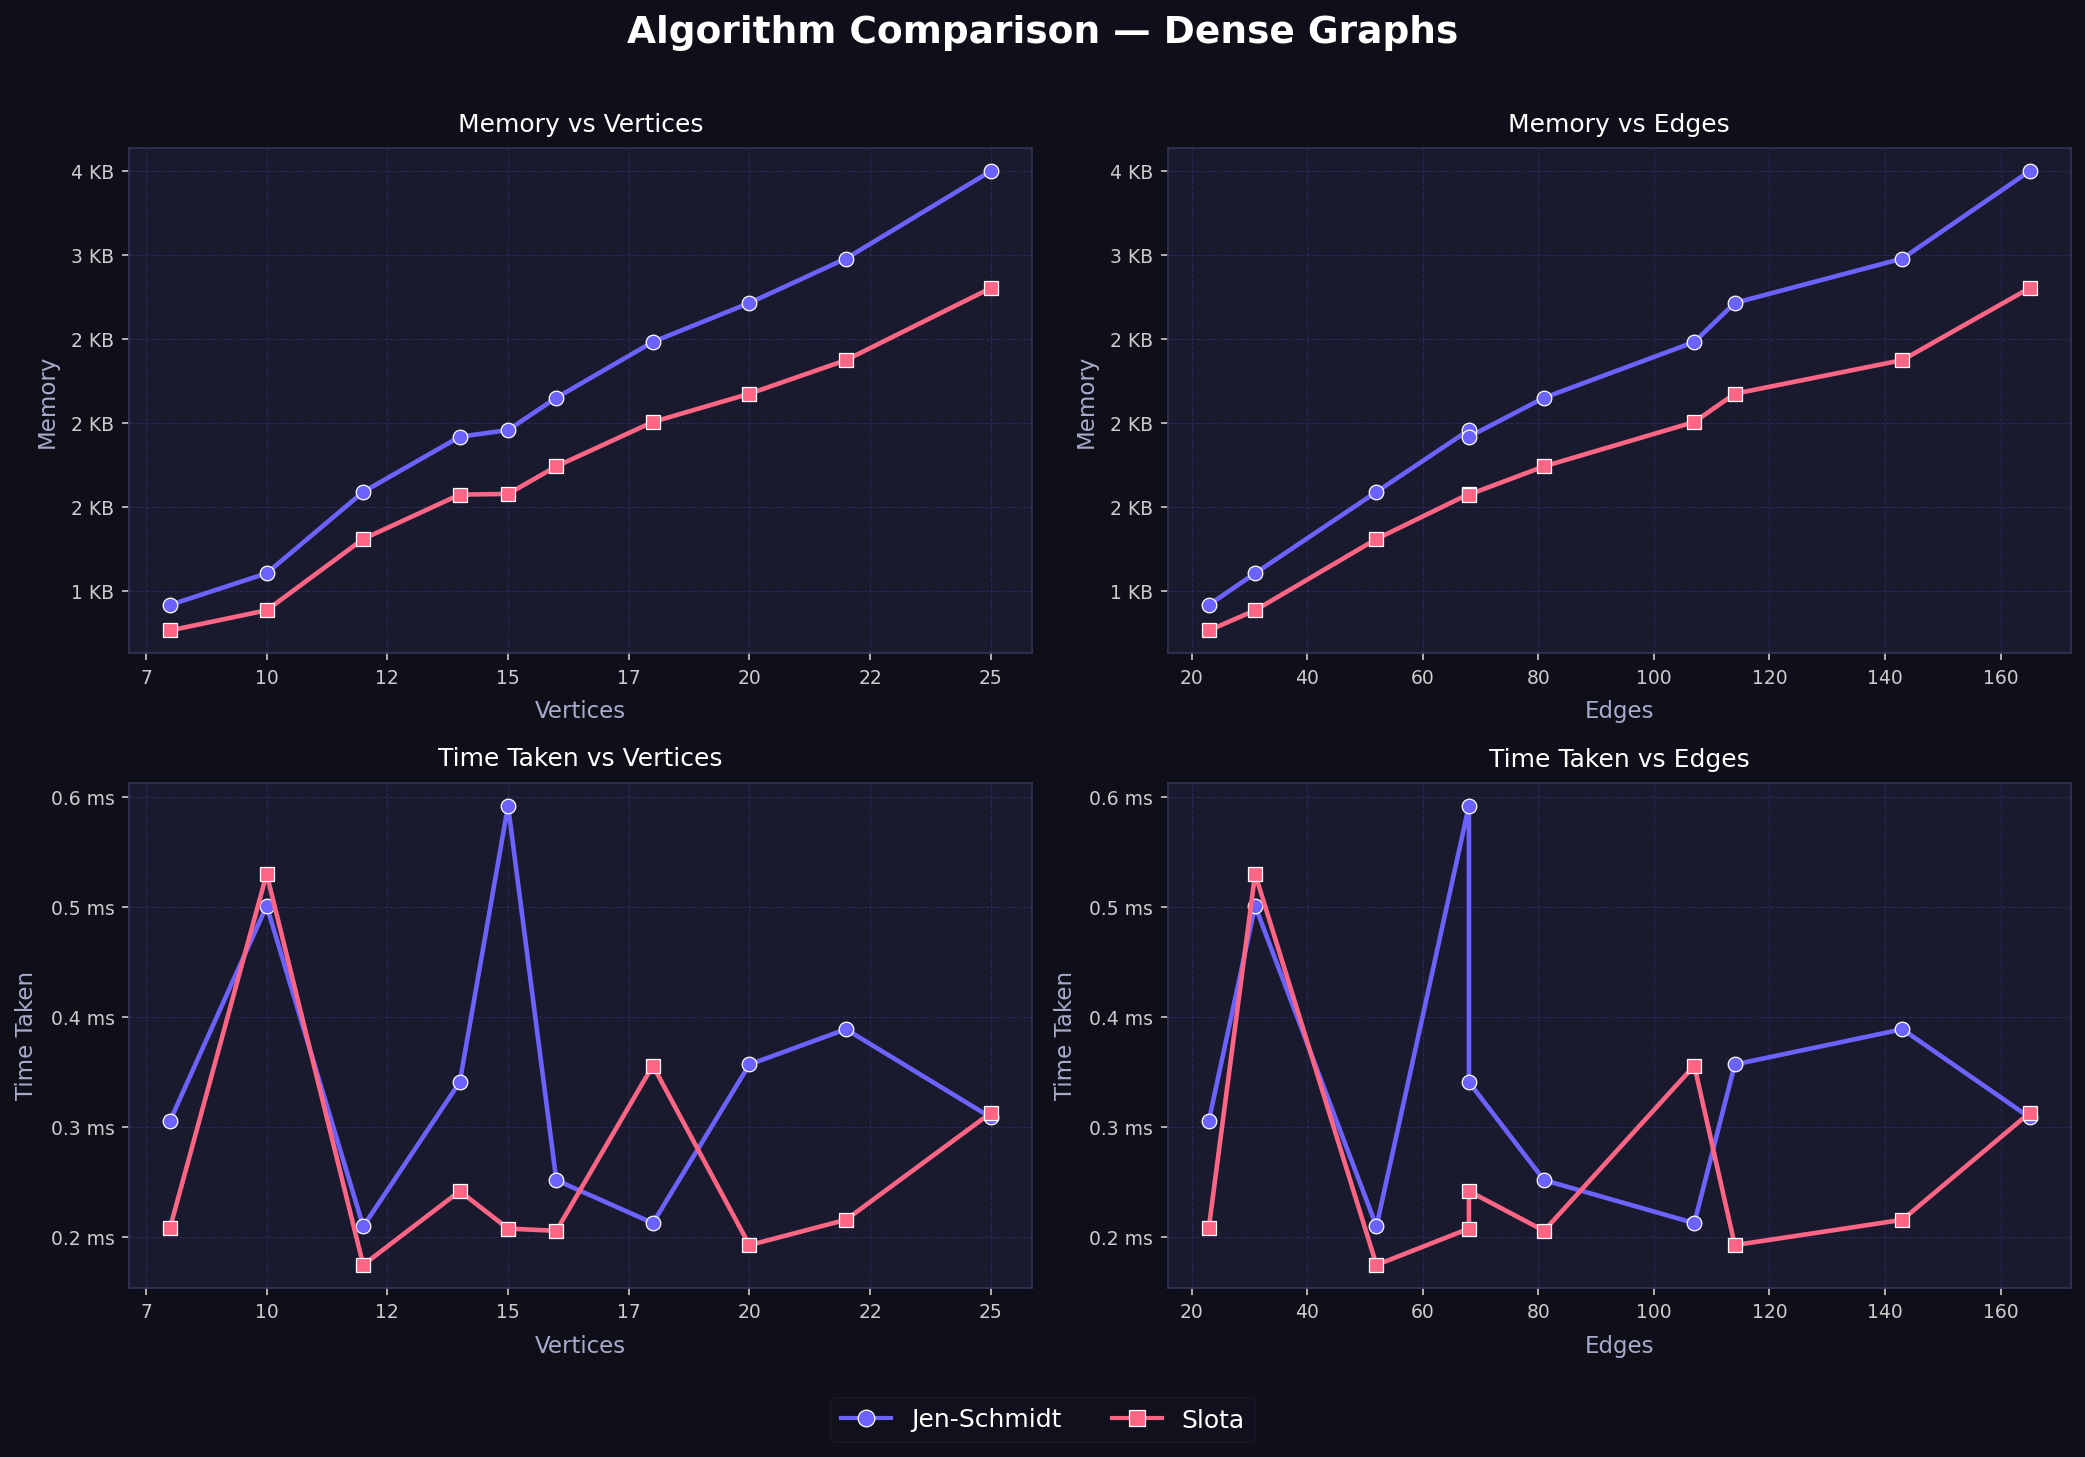
\includegraphics[width=0.9\textwidth]{plots/dense.png}
    \caption{Dense graphs: JS memory gap grows with edge count.}
\end{figure}

\begin{figure}[h]
    \centering
    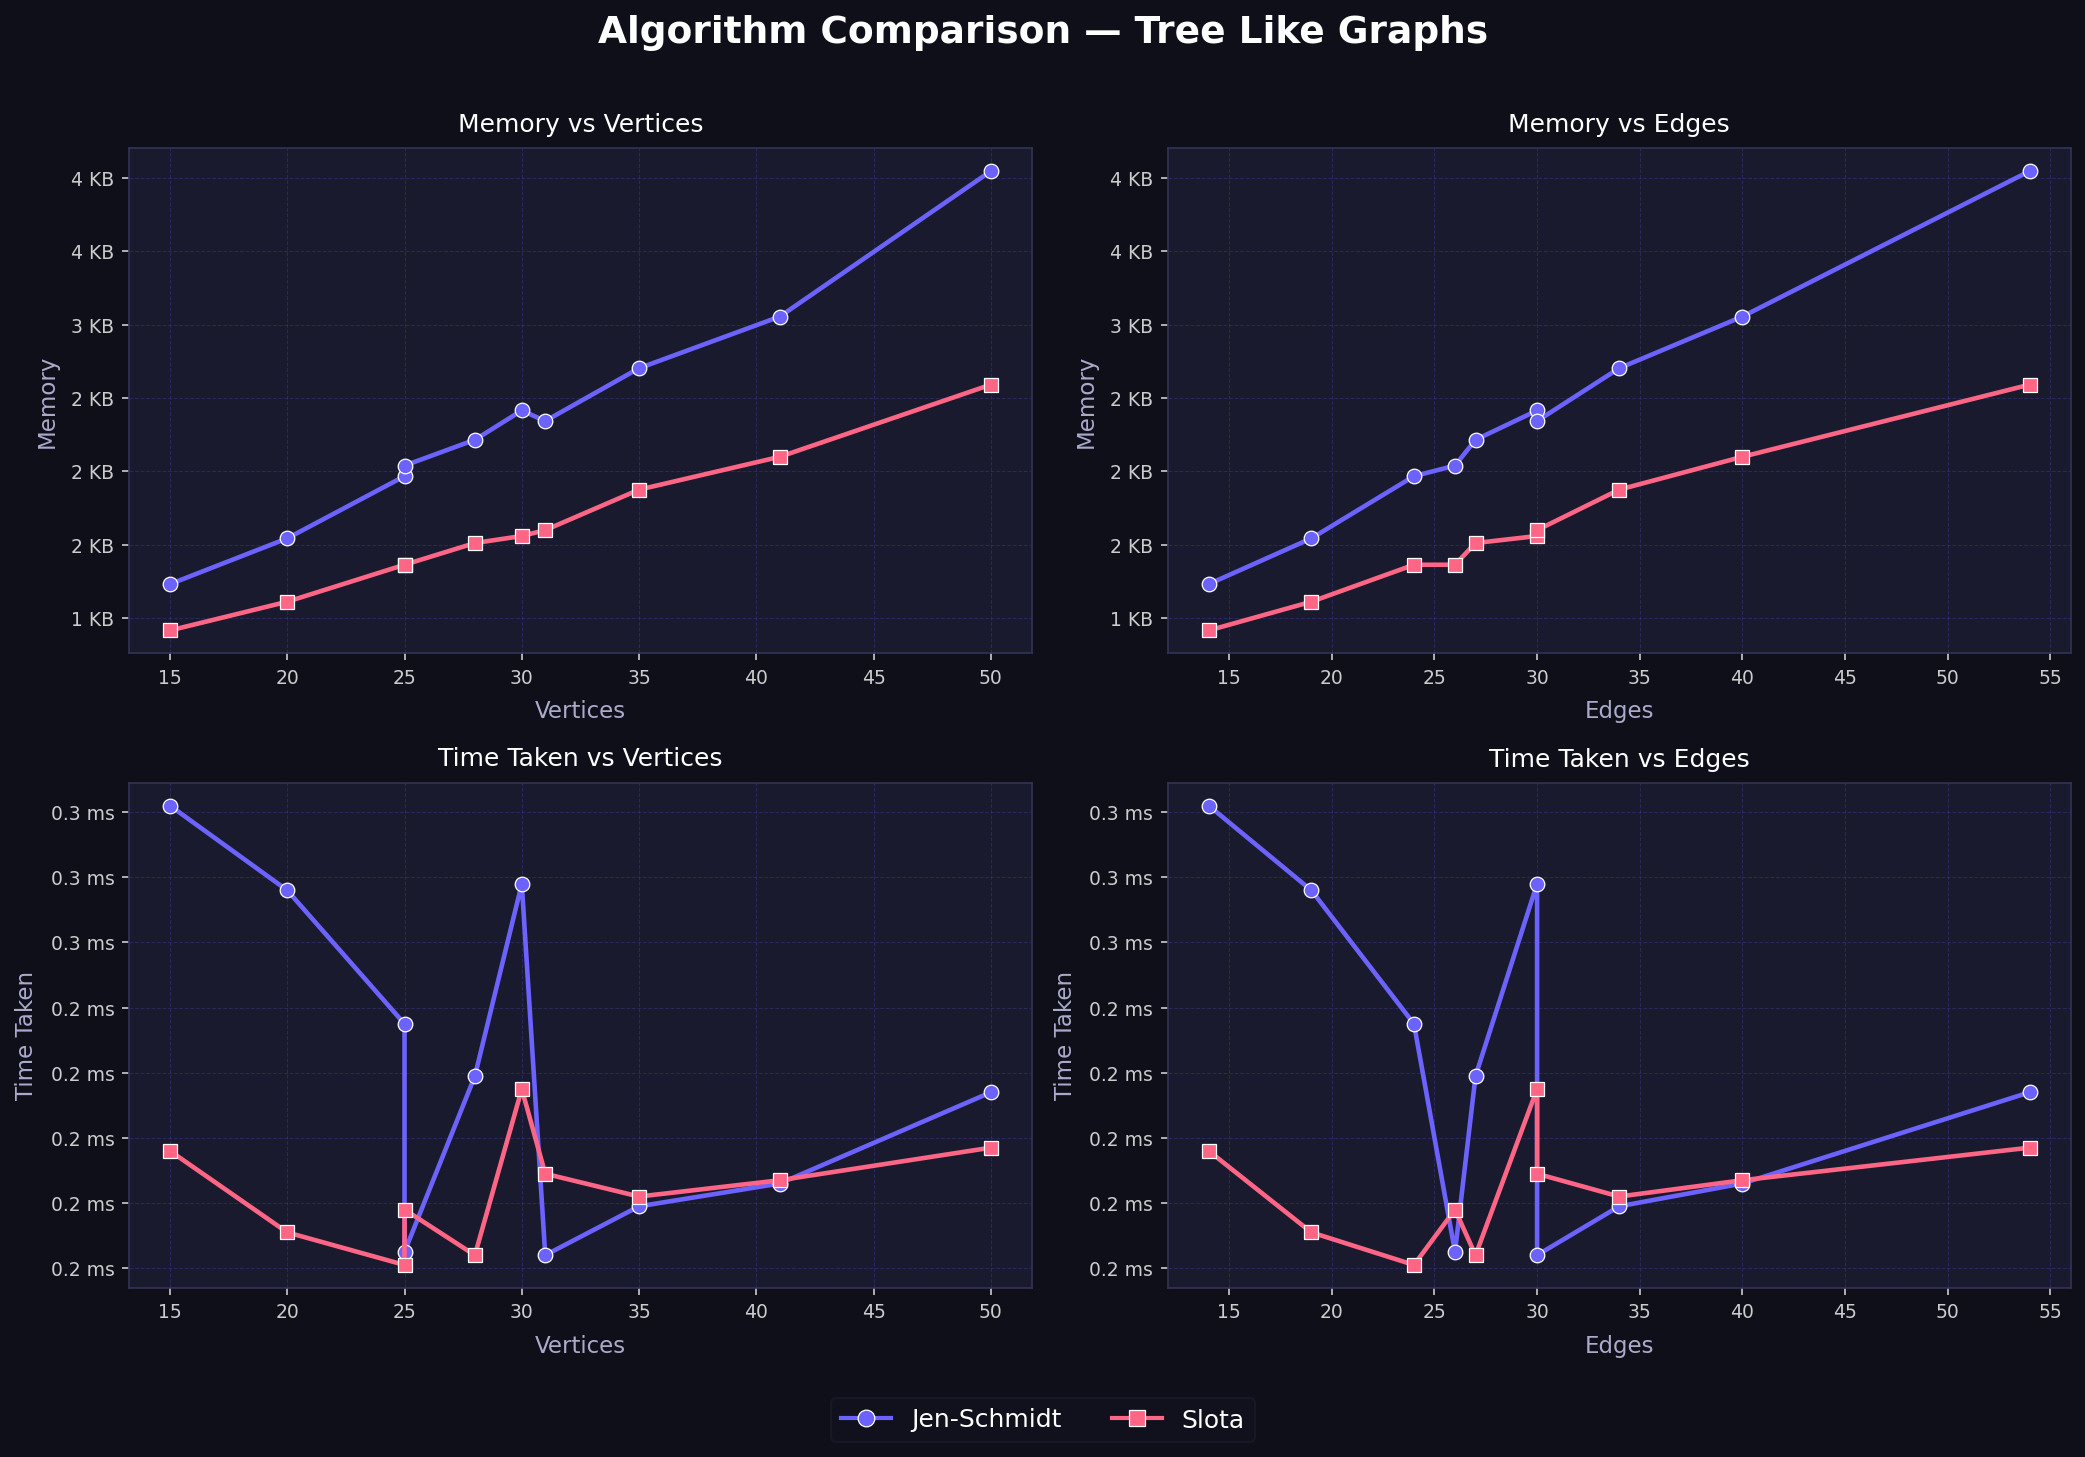
\includegraphics[width=0.9\textwidth]{plots/tree_like.png}
    \caption{Tree-like graphs: Slota performs more exclusion-BFS calls.}
\end{figure}


% =============================================================================
\section{Conclusion}
% =============================================================================

Both algorithms achieve practical $O(V+E)$ performance across all tested
graph families.

\textbf{Slota--Madduri} is preferred when memory efficiency matters (it
uses 20--40\% less) or when the input is dense/highly connected (its early
BFS termination gives a speed advantage of 25--40\%).

\textbf{Jens-Schmidt} is preferred when a strict $O(V+E)$ time guarantee
is required regardless of topology, when the graph is sparse or
tree-structured (where Slota's worst case manifests), or when the ear
decomposition itself is a required output.

For general-purpose biconnectivity testing on large social/web graphs,
Slota--Madduri is the better engineered choice.  For robustness and
structural certification, Jens-Schmidt is the algorithm of choice.


% =============================================================================
\begin{thebibliography}{9}
\bibitem{jenschmidt}
    J.\ M.\ Schmidt,
    \textit{A simple test on 2-vertex- and 2-edge-connectivity},
    Information Processing Letters, 113(7):241--244, 2013.

\bibitem{slota}
    G.\ Slota and K.\ Madduri,
    \textit{Simple Parallel Biconnectivity Algorithms for Multicore Platforms},
    IEEE 21st International Conference on High Performance Computing (HiPC), 2014.
\end{thebibliography}

\end{document}
